\documentclass[11pt]{article}
% Style of the NETRA operator guide (Indonesian). Same palette as the dashboard.
\usepackage[a4paper,margin=2.2cm,headheight=14pt,includehead,includefoot]{geometry}
\usepackage[T1]{fontenc}
\usepackage[utf8]{inputenc}
\usepackage{mathptmx}
\usepackage[scaled=0.92]{helvet}
\usepackage{courier}
\renewcommand{\familydefault}{\sfdefault}
\usepackage{microtype}
\usepackage{xcolor}
\usepackage{graphicx}
\usepackage{booktabs,tabularx,array}
\usepackage{enumitem}
\usepackage{amssymb}
\usepackage{pifont}
\usepackage{tikz}
\usetikzlibrary{arrows.meta,positioning,shapes.geometric,fit,backgrounds,calc}
\usepackage{titlesec}
\usepackage{fancyhdr}
\usepackage[most]{tcolorbox}
\usepackage{multicol}
\usepackage{float}
\usepackage[hidelinks]{hyperref}
\usepackage{bookmark}

\definecolor{netra}{HTML}{0E7490}
\definecolor{netralight}{HTML}{E6F6FA}
\definecolor{ink}{HTML}{0F172A}
\definecolor{muted}{HTML}{64748B}
\definecolor{line}{HTML}{CBD5E1}
\definecolor{warnc}{HTML}{B45309}
\definecolor{okc}{HTML}{15803D}
\definecolor{dangerc}{HTML}{B91C1C}

\hypersetup{colorlinks=true,linkcolor=netra,urlcolor=netra,
  pdftitle={NETRA - Panduan Operator},pdfauthor={EZRA Robotics},pdfsubject={Robot patroli Genisom L1W dan pusat komando NETRA}}

% Indonesian names without babel (no Indonesian hyphenation patterns installed); text is set
% ragged right without hyphenation, which reads better for a step-by-step guide anyway.
\renewcommand{\contentsname}{Daftar Isi}
\renewcommand{\figurename}{Gambar}
\renewcommand{\tablename}{Tabel}
\hyphenpenalty=10000
\exhyphenpenalty=10000
\AtBeginDocument{\raggedright}
\setlength{\parindent}{0pt}
\setlength{\parskip}{5pt}
\renewcommand{\arraystretch}{1.25}
\setlist{itemsep=2pt,topsep=3pt}
\setlist[enumerate]{label=\textbf{\color{netra}\arabic*.},leftmargin=1.6em}
\setlist[itemize]{label=\textcolor{netra}{\textbullet},leftmargin=1.4em}

\titleformat{\section}{\sffamily\bfseries\LARGE\color{netra}}{\thesection}{0.6em}{}
\titlespacing*{\section}{0pt}{6pt}{10pt}
\titleformat{\subsection}{\sffamily\bfseries\large\color{ink}}{\thesubsection}{0.6em}{}
\titlespacing*{\subsection}{0pt}{12pt}{4pt}
\titleformat{\subsubsection}{\sffamily\bfseries\color{netra}}{}{0pt}{}

\pagestyle{fancy}
\fancyhf{}
\fancyhead[L]{\small\color{netra}\textbf{NETRA}\enspace\color{muted}Panduan Operator}
\fancyhead[R]{\small\color{muted}\nouppercase{\leftmark}}
\fancyfoot[L]{\small\color{muted}EZRA Robotics}
\fancyfoot[R]{\small\color{muted}\thepage}
\renewcommand{\headrulewidth}{0.4pt}
\fancypagestyle{plain}{}  % pages that ask for "plain" (table of contents) keep the same header
\renewcommand{\headrule}{\color{line}\hrule height\headrulewidth}
\renewcommand{\sectionmark}[1]{\markboth{#1}{}}

% UI labels and keys
\newcommand{\ui}[1]{\textbf{#1}}
\newcommand{\key}[1]{\tikz[baseline=(k.base)]\node[draw=muted,rounded corners=2pt,inner sep=2pt,font=\footnotesize\bfseries](k){#1};}
\newcommand{\code}[1]{\texttt{\small #1}}

% Boxes
\newtcolorbox{penting}[1][Penting]{colback=red!4,colframe=dangerc,fonttitle=\bfseries\small,title=#1,
  boxrule=0.7pt,arc=2pt,left=7pt,right=7pt,top=4pt,bottom=4pt,before skip=8pt,after skip=8pt}
\newtcolorbox{tips}[1][Tips]{colback=netralight,colframe=netra,fonttitle=\bfseries\small,title=#1,
  boxrule=0.7pt,arc=2pt,left=7pt,right=7pt,top=4pt,bottom=4pt,before skip=8pt,after skip=8pt}
\newtcolorbox{teknisi}[1][Untuk teknisi]{colback=gray!5,colframe=muted,fonttitle=\bfseries\small,title=#1,
  boxrule=0.6pt,arc=2pt,left=7pt,right=7pt,top=4pt,bottom=4pt,before skip=8pt,after skip=8pt}

% Screenshot with a thin frame and a caption line under it
\setlength{\fboxsep}{0pt}
\newcommand{\shot}[3][\linewidth]{%
  \begin{center}
    \fcolorbox{line}{white}{\includegraphics[width=\dimexpr#1-1pt\relax]{img/#2}}\\[3pt]
    {\small\color{muted}#3}
  \end{center}}

% Numbered call-out marker used in text and on top of screenshots
\newcommand{\callout}[1]{\tikz[baseline=(c.base)]\node[circle,fill=netra,text=white,inner sep=1.2pt,minimum size=13pt,font=\scriptsize\bfseries](c){#1};}

\tikzset{
  box/.style={draw=netra,fill=netralight,rounded corners=4pt,align=center,font=\small,minimum height=12mm,inner sep=5pt},
  dark/.style={draw=ink,fill=ink!6,rounded corners=4pt,align=center,font=\small,minimum height=12mm,inner sep=5pt},
  ext/.style={draw=muted,fill=gray!6,rounded corners=4pt,align=center,font=\small,minimum height=12mm,inner sep=5pt,dashed},
  arr/.style={-{Stealth[length=2.4mm]},thick,draw=ink!70},
  biarr/.style={{Stealth[length=2.4mm]}-{Stealth[length=2.4mm]},thick,draw=ink!70},
  lbl/.style={font=\scriptsize,fill=white,inner sep=1.5pt,text=muted},
  state/.style={draw=#1,fill=#1!8,rounded corners=3pt,font=\small\bfseries,inner sep=5pt,text=#1!70!black},
}
\setlength{\emergencystretch}{3em}

% Table columns set ragged right like the text: Y (flexible), B{width} (bold first column)
\newcolumntype{Y}{>{\raggedright\arraybackslash}X}
\newcolumntype{B}[1]{>{\raggedright\arraybackslash\bfseries}p{#1}}

% Compact table of contents: one line per section, on the first page with the introduction
\usepackage{tocloft}
\setlength{\cftbeforesecskip}{2.5pt}
\renewcommand{\cftsecfont}{\color{ink}}
\renewcommand{\cftsecpagefont}{\color{muted}}
\renewcommand{\cftsecleader}{\cftdotfill{\cftdotsep}}
\setlength{\cftbeforetoctitleskip}{8pt}
\setlength{\cftaftertoctitleskip}{6pt}
\renewcommand{\cfttoctitlefont}{\sffamily\bfseries\LARGE\color{netra}}


\newcommand{\ra}{\ensuremath{\rightarrow}}
\newcommand{\gtq}{\ensuremath{\geq}}

\begin{document}

% ------------------------------------------------------------------------------------------ cover
\begin{titlepage}
\thispagestyle{empty}

\begin{tikzpicture}[remember picture,overlay]
  \fill[netra] (current page.north west) rectangle ([yshift=-10.5cm]current page.north east);
  \fill[netra!80!black] ([yshift=-10.5cm]current page.north west) rectangle ([yshift=-10.8cm]current page.north east);
  \node[anchor=north west,text=white,font=\fontsize{54}{60}\selectfont\bfseries] at ([xshift=2.2cm,yshift=-3.2cm]current page.north west) {\textls[350]{NETRA}};
  \node[anchor=north west,text=white!85!netra,font=\Large] at ([xshift=2.25cm,yshift=-5.5cm]current page.north west) {\textls[120]{PUSAT KOMANDO PATROLI}};
  \node[anchor=north west,text=ink,font=\fontsize{34}{40}\selectfont\bfseries] at ([xshift=2.2cm,yshift=-13cm]current page.north west) {Panduan Operator};
  \node[anchor=north west,text width=15cm,text=muted,font=\Large] at ([xshift=2.2cm,yshift=-15cm]current page.north west)
    {Menjalankan robot patroli Genisom L1W dan pusat komando NETRA, langkah demi langkah, untuk petugas tanpa latar belakang teknik.};
  \node[anchor=south west,font=\Large] at ([xshift=2.2cm,yshift=2.6cm]current page.south west)
    {\textcolor{ink}{\textbf{\textls[200]{EZRA}}}\,\textcolor{muted}{\small\textls[200]{ROBOTICS}}};
  \node[anchor=south east,text=muted,font=\small,align=right] at ([xshift=-2.2cm,yshift=2.65cm]current page.south east)
    {Versi 1.0 \textperiodcentered{} Oktober 2026};
  \draw[line,line width=0.6pt] ([xshift=2.2cm,yshift=2.2cm]current page.south west) -- ([xshift=-2.2cm,yshift=2.2cm]current page.south east);
\end{tikzpicture}
\end{titlepage}

% ------------------------------------------------------------------------------------------ intro
\section*{Tentang panduan ini}
\markboth{Tentang panduan ini}{}
Panduan ini untuk petugas yang menjalankan patroli robot setiap hari: operator, petugas keamanan dan
supervisor. Anda tidak perlu mengerti teknik robot. Ikuti langkah bernomor, perhatikan kotak merah
\ui{Penting}, dan simpan \hyperref[sec:kartu]{kartu ringkas} di halaman terakhir di dekat meja kontrol.

Bagian yang hanya untuk teknisi diberi kotak abu-abu \ui{Untuk teknisi}. Gambar layar memakai bahasa
Indonesia (tombol \ui{ID} di kanan atas NETRA) dan mode terang; data di gambar hanya contoh.

\setcounter{tocdepth}{1}
\tableofcontents
\clearpage

% ------------------------------------------------------------------------------------------ 1
\section{Mengenal sistem}

\subsection{Apa yang dikerjakan robot}
\begin{itemize}
  \item Robot berjalan sendiri menyusuri \ui{rute} yang sudah direkam sebelumnya, sesuai jadwal atau
        saat diperintah dari NETRA.
  \item Di setiap \ui{titik stop} robot berhenti sebentar dan memeriksa lantai dengan kamera dan AI:
        sampah, tumpahan, lantai rusak dan orang terjatuh.
  \item Temuan (\ui{anomali}) dikirim ke NETRA lengkap dengan foto dan posisinya. Petugas memastikan
        temuan itu benar (\ui{validasi}), lalu NETRA bisa meneruskannya ke grup Telegram, misalnya
        grup cleaning service.
  \item Robot menghitung orang di sekitarnya untuk peta keramaian.
  \item Bila ada orang atau barang di jalur, robot menghindar dengan bergeser ke samping, atau berhenti
        dan menunggu sampai jalur bebas.
\end{itemize}

\subsection{Tiga bagian sistem}
\begin{center}
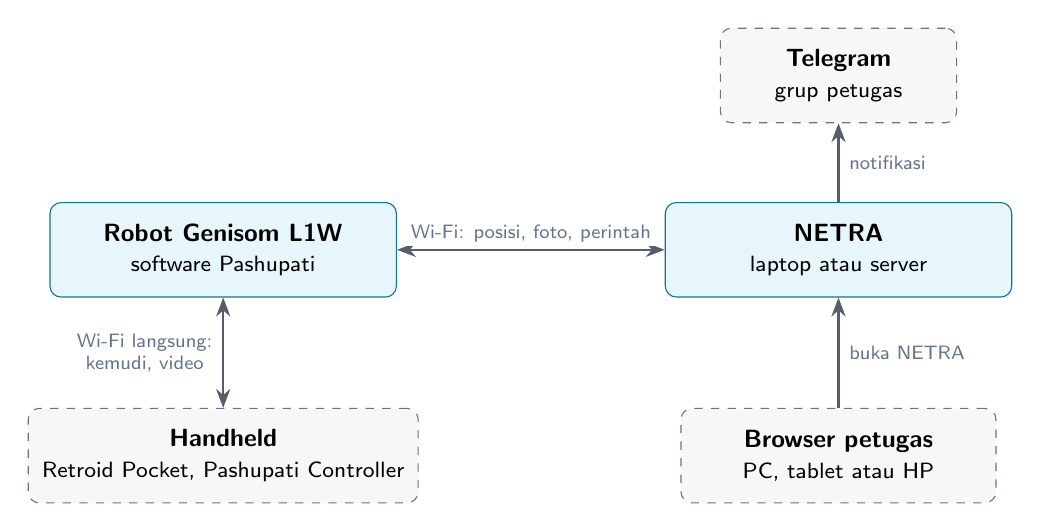
\begin{tikzpicture}[node distance=12mm and 16mm]
  \node[box,minimum width=44mm] (robot) {\textbf{Robot Genisom L1W}\\\footnotesize software Pashupati};
  \node[box,minimum width=44mm,right=34mm of robot] (netra) {\textbf{NETRA}\\\footnotesize laptop atau server};
  \node[ext,minimum width=40mm,below=14mm of robot] (pad) {\textbf{Handheld}\\\footnotesize Retroid Pocket, Pashupati Controller};
  \node[ext,minimum width=40mm,below=14mm of netra] (browser) {\textbf{Browser petugas}\\\footnotesize PC, tablet atau HP};
  \node[ext,minimum width=30mm,above=10mm of netra] (tg) {\textbf{Telegram}\\\footnotesize grup petugas};
  \draw[biarr] (robot) -- node[lbl,above=1pt] {Wi-Fi: posisi, foto, perintah} (netra);
  \draw[biarr] (pad) -- node[lbl,left=2pt,align=center] {Wi-Fi langsung:\\kemudi, video} (robot);
  \draw[arr] (browser) -- node[lbl,right=2pt] {buka NETRA} (netra);
  \draw[arr] (netra) -- node[lbl,right=2pt] {notifikasi} (tg);
\end{tikzpicture}
\end{center}

\begin{tabularx}{\linewidth}{@{}B{3.4cm}YY@{}}
\toprule
Bagian & Apa itu & Dipakai untuk \\
\midrule
Robot Genisom L1W & Robot berkaki empat beroda dengan sensor LiDAR (jarak 360\textdegree) dan kamera, menjalankan software patroli Pashupati & Patroli, inspeksi lantai, menghitung orang \\
NETRA & Pusat komando berbasis web yang berjalan di laptop atau server & Memantau, memulai patroli, validasi anomali, jadwal, laporan \\
Handheld & Aplikasi Pashupati Controller di Retroid Pocket, tersambung langsung ke robot & Mengemudikan robot, berdiri dan duduk, merekam rute, rem darurat di lapangan \\
\bottomrule
\end{tabularx}

\subsection{Peran pengguna}
Setiap orang masuk ke NETRA dengan akun sendiri. Menu dan tombol yang tidak sesuai peran tidak tampil.

\begin{tabularx}{\linewidth}{@{}B{3.4cm}Y@{}}
\toprule
Peran & Boleh \\
\midrule
Pemantau & Melihat semua halaman \\
Operator & Menjalankan patroli, mengendalikan robot, memvalidasi anomali \\
Supervisor & Seperti operator, ditambah robot, aturan anomali, denah dan log audit \\
Admin & Semuanya, termasuk pengguna dan klien API \\
\bottomrule
\end{tabularx}

% ------------------------------------------------------------------------------------------ 2
\section{Keselamatan}
\label{sec:safety}

\subsection{Aturan dasar}
\begin{itemize}
  \item Jaga jarak minimal 1 meter dari robot yang bergerak. Jangan berdiri tepat di depannya.
  \item Jangan menyentuh, mendorong, menduduki atau menaiki robot, dan jangan menaruh barang di atasnya.
  \item Jangan menutupi sensor dan kamera robot.
  \item Jalankan robot hanya di lantai datar pada rute. Jangan bawa robot ke tangga, eskalator,
        travelator atau lantai basah dan licin.
  \item Awasi anak-anak dan hewan di dekat robot.
  \item Saat memindahkan robot dengan handheld, kemudikan pelan dan pastikan jalur kosong.
  \item Menyalakan, mematikan dan mengisi daya robot hanya sesuai buku manual Genisom L1W.
\end{itemize}

Robot sendiri melambat dan berhenti bila ada orang atau benda terlalu dekat (\ui{area aman}). Fitur ini
membantu, tetapi tidak menggantikan pengawasan petugas.

\subsection{Rem darurat}
\ui{Rem darurat} (e-stop) menahan robot diam di tempat. Selama aktif, robot tidak menerima perintah
gerak apa pun, baik dari NETRA maupun dari handheld. Rem tetap aktif sampai seseorang sengaja
melepasnya (\hyperref[sec:estop]{bagian 8}).

\begin{tabularx}{\linewidth}{@{}B{3.4cm}Y@{}}
\toprule
Dari & Caranya \\
\midrule
Handheld & Tombol merah \ui{STOP} di layar, atau tombol \key{B} \\
NETRA & Tombol merah \ui{Rem darurat} di kartu robot (Dasbor atau Peta operasi) \\
\bottomrule
\end{tabularx}

\begin{penting}
Kalau ragu, tekan rem darurat. Robot berhenti seketika dan tidak ada yang rusak. Lebih baik berhenti
tanpa perlu daripada terlambat berhenti.
\end{penting}

% ------------------------------------------------------------------------------------------ 3
\section{Persiapan sebelum patroli}
\label{sec:prep}
Lakukan langkah ini setiap awal shift, atau sebelum patroli pertama hari itu.

\begin{enumerate}
  \item \textbf{Pusat komando menyala.} Buka NETRA di browser (bagian~\ref{sec:login}). Bila halaman
        tidak terbuka, hubungi teknisi.
  \item \textbf{Area aman.} Lantai rute kering, tidak ada kabel atau barang di jalur, pintu yang
        dilewati terbuka.
  \item \textbf{Baterai.} Robot terisi daya. Mulailah patroli dengan baterai di atas 50\,\%.
  \item \textbf{Nyalakan robot} sesuai buku manual Genisom L1W. Software patroli menyala sendiri.
        Tunggu 1--3 menit sampai kartu robot di NETRA menunjukkan titik hijau (online) dan angka
        \ui{Robot aktif} di bagian atas bertambah.
  \item \textbf{Nyalakan handheld}, buka aplikasi \ui{Pashupati Controller} dan pilih robot di daftar
        (biasanya \ui{Robot utama}). Layar menampilkan video kamera dan peta.
  \item \textbf{Berdirikan robot}: ikon \ui{Berdiri} di bawah tombol STOP, atau \key{L1}\,+\,\key{A}.
        Aplikasi meminta konfirmasi karena robot akan bergerak sendiri.
  \item \textbf{Bawa robot ke titik awal rute.} Pindah ke \ui{REMOTE} (tombol \key{Start}), lalu
        kemudikan pelan: stik kiri untuk maju, mundur dan bergeser, stik kanan untuk berbelok.
        Hadapkan kamera robot ke \ui{AprilTag} di titik awal, yaitu kertas bermotif kotak hitam-putih
        yang ditempel di dinding atau tiang.
  \item \textbf{Lokalisasi}: tekan \ui{Lokalisasi} di kartu robot NETRA, atau \ui{Lokasi} di handheld.
        Tunggu sampai handheld menulis \ui{Terlokalisasi} atau \ui{Tag}. Tanpa lokalisasi, robot
        menolak memulai patroli.
  \item \textbf{Kembali ke AUTO} (tombol \key{Start}). Di mode REMOTE robot hanya mengikuti stik dan
        tidak berpatroli.
\end{enumerate}

\begin{tips}
Robot boleh mulai dari samping rute; ia akan berjalan masuk ke rute sendiri. Bila robot terlalu jauh
dari rute, patroli ditolak: dekatkan robot dulu dengan handheld.
\end{tips}

% ------------------------------------------------------------------------------------------ 4
\section{Masuk ke NETRA}
\label{sec:login}

\subsection{Login}
\begin{minipage}[t]{0.52\linewidth}
\vspace{0pt}\raggedright
\begin{enumerate}
  \item Buka browser (Chrome, Edge atau Safari) ke alamat NETRA dari admin, misalnya
        \code{https://netra.contoh.com}, atau di jaringan robot \code{http://192.168.234.35}.
  \item Isi \ui{Nama pengguna} dan \ui{Kata sandi}, lalu tekan \ui{Masuk}.
  \item Pilih bahasa \ui{ID} di kanan atas. Pilihan ini diingat di browser tersebut.
\end{enumerate}
Setelah 8 kali salah kata sandi, login ditahan 10 menit. Lupa kata sandi? Minta admin
mereset di menu \ui{Pengguna}.
\end{minipage}\hfill
\begin{minipage}[t]{0.42\linewidth}
\vspace{0pt}\raggedright
\centering
\fcolorbox{line}{white}{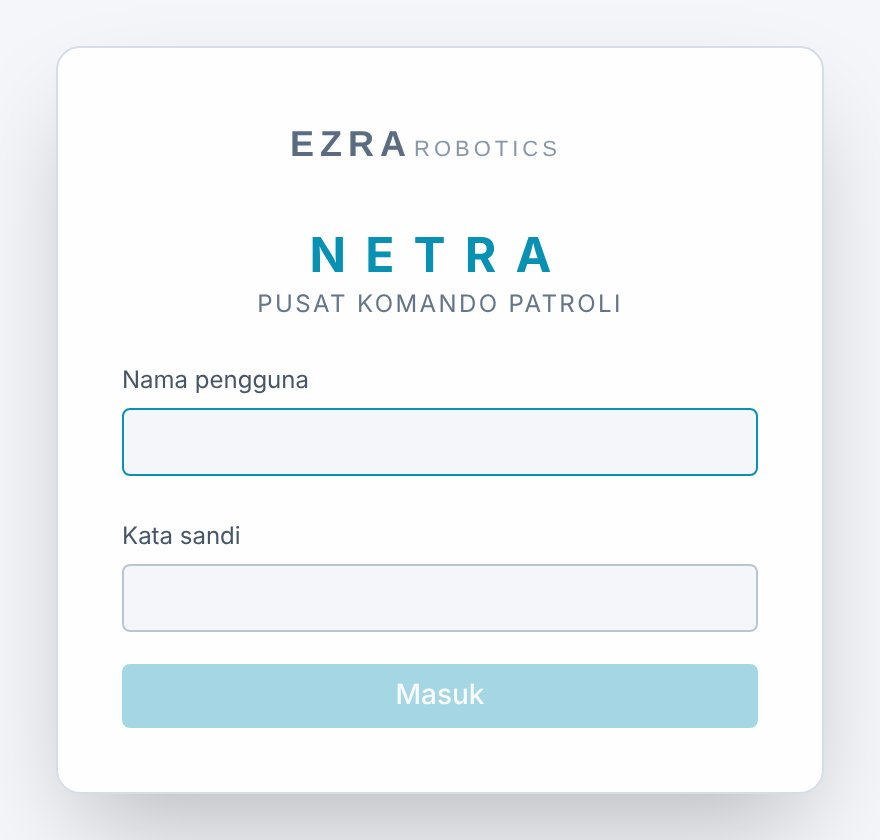
\includegraphics[width=\dimexpr\linewidth-1pt\relax]{img/login}}\\[3pt]
{\small\color{muted}Halaman login}
\end{minipage}

\subsection{Bagian layar}
\begin{itemize}
  \item \textbf{Bilah atas}: tombol sembunyikan menu (atau tombol \key{[}), status koneksi
        (\textcolor{okc}{\ui{Terhubung}} hijau, \textcolor{dangerc}{\ui{Terputus}} merah), jumlah robot
        aktif, jam, layar penuh, mode terang/gelap dan bahasa.
  \item \textbf{Menu kiri}, dikelompokkan seperti tabel di bawah.
  \item \textbf{Kiri bawah}: nama Anda, tombol ganti kata sandi (ikon kunci) dan tombol keluar.
\end{itemize}

\begin{tabularx}{\linewidth}{@{}B{3.2cm}Y@{}}
\toprule
Menu & Isi \\
\midrule
Dasbor & Ringkasan hari ini, peta langsung, kontrol robot, hal yang perlu perhatian \\
Peta operasi & Peta besar dengan robot, rute, anomali dan keramaian \\
Anomali & Semua temuan robot dan validasinya \\
Patroli & Riwayat patroli, laporan per patroli, mulai patroli \\
Jadwal & Patroli otomatis per hari dan jam \\
Rute & Rute yang sudah direkam robot \\
Keramaian & Peta dan grafik jumlah orang \\
Laporan & Laporan PDF dan Excel untuk periode apa pun \\
Denah & Denah mall dan kalibrasinya (supervisor) \\
Pengaturan, Pengguna, Log audit & Administrasi (supervisor dan admin) \\
\bottomrule
\end{tabularx}

\begin{tips}
Untuk layar dinding di ruang kontrol: buka \ui{Dasbor}, tekan tombol layar penuh dan pilih mode gelap.
\end{tips}

% ------------------------------------------------------------------------------------------ 5
\clearpage
\section{Dasbor}
Dasbor adalah halaman utama selama bertugas.

\begin{center}
\begin{tikzpicture}
  \node[anchor=south west,inner sep=0,draw=line] (img) at (0,0) {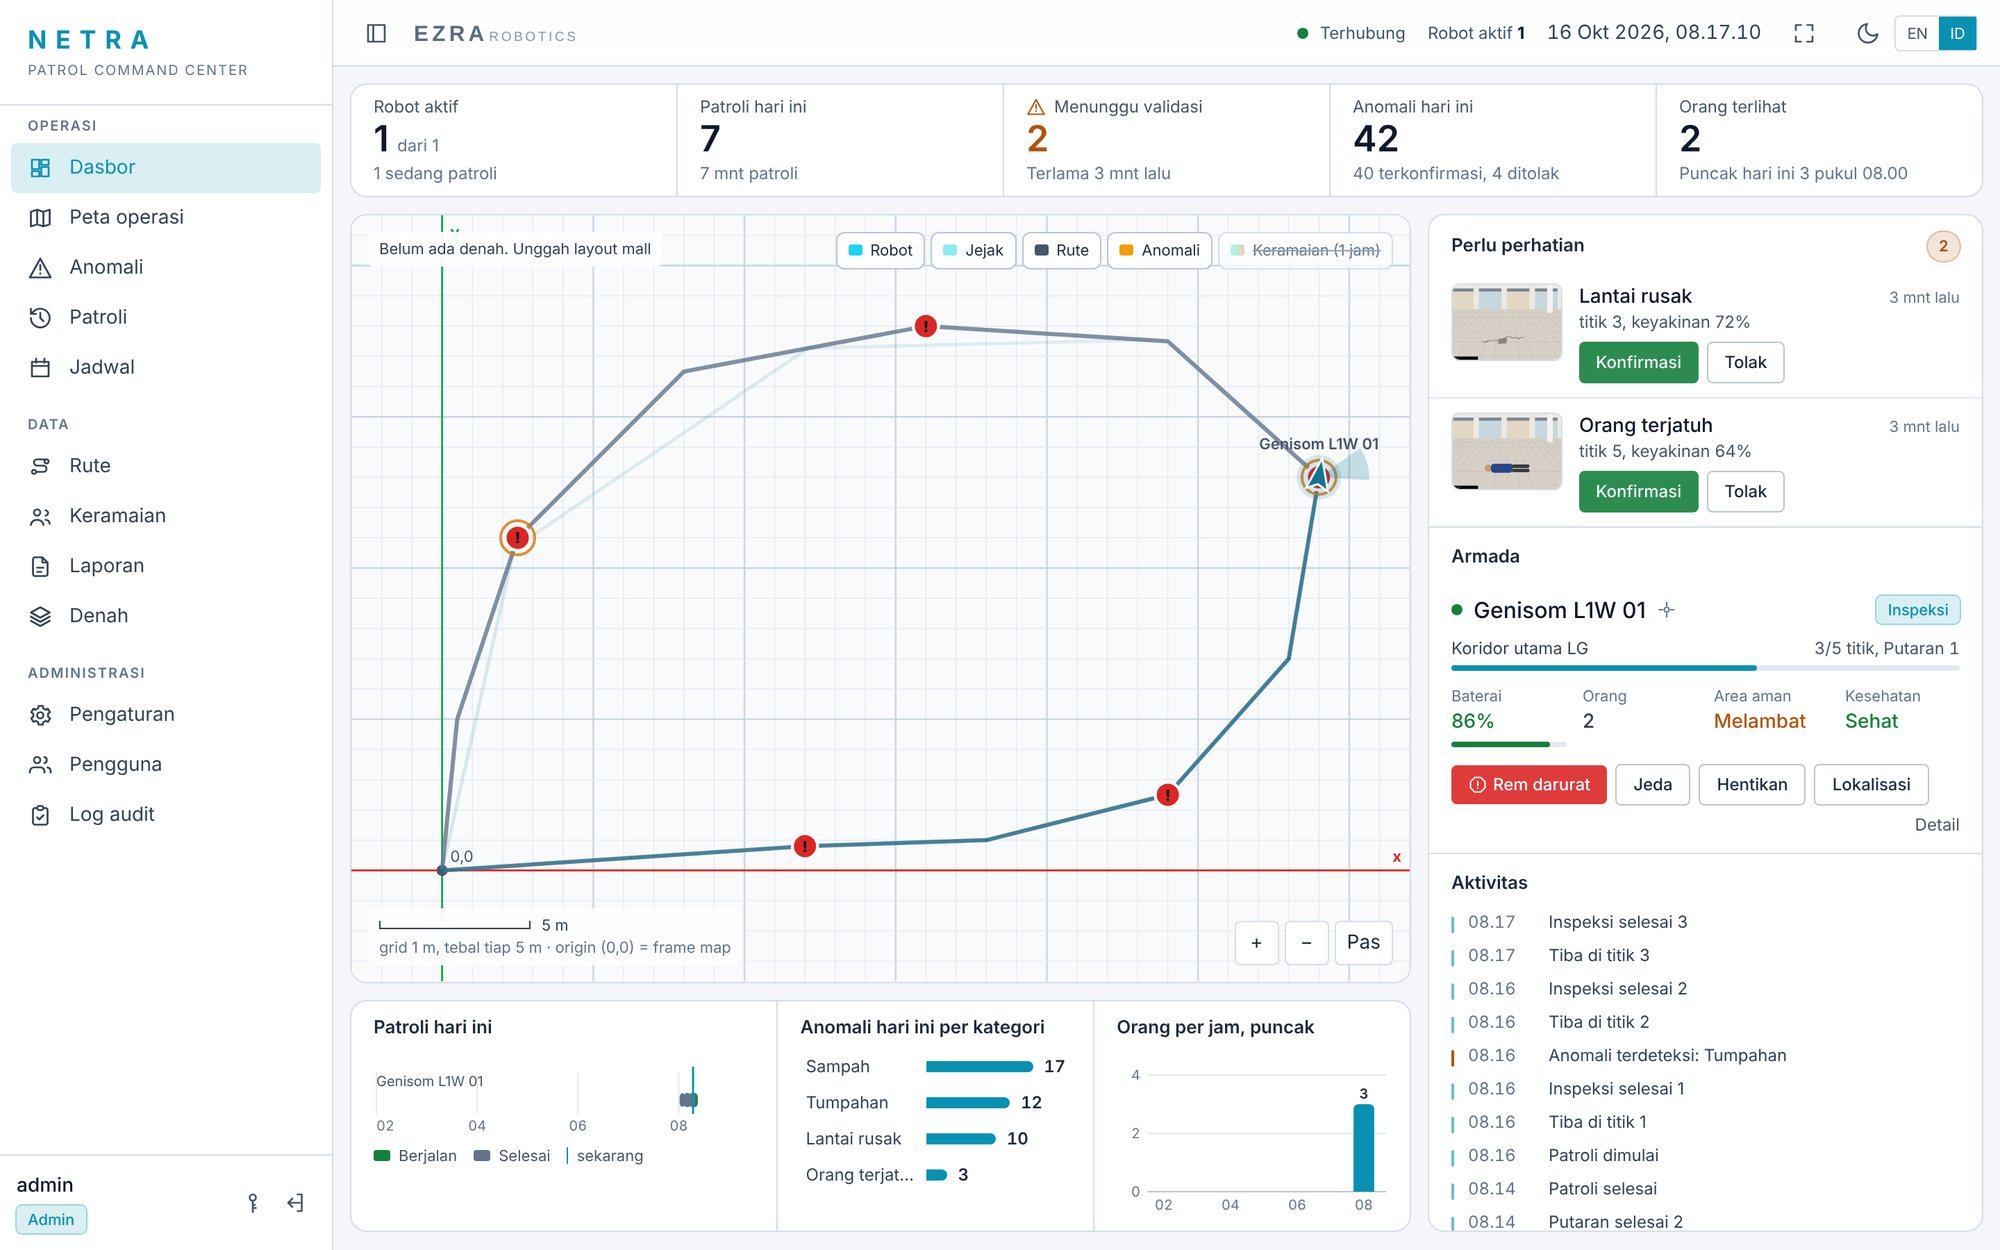
\includegraphics[width=\linewidth]{img/dashboard}};
  \begin{scope}[x={(img.south east)},y={(img.north west)}]
    \node at (0.167,0.885) {\callout{1}};
    \node at (0.190,0.760) {\callout{2}};
    \node at (0.413,0.800) {\callout{3}};
    \node at (0.818,0.805) {\callout{4}};
    \node at (0.778,0.556) {\callout{5}};
    \node at (0.782,0.327) {\callout{6}};
    \node at (0.258,0.178) {\callout{7}};
  \end{scope}
\end{tikzpicture}\\[3pt]
{\small\color{muted}Dasbor saat robot berpatroli}
\end{center}

\begin{itemize}[leftmargin=2em,labelsep=0.6em]
  \item[\callout{1}] \textbf{Angka ringkas}: robot aktif, patroli hari ini, anomali yang \ui{Menunggu validasi},
        anomali hari ini dan orang yang terlihat robot sekarang.
  \item[\callout{2}] \textbf{Peta langsung}: robot (panah menunjukkan arah hadap), jejak yang baru dilalui, rute yang
        sedang dipatroli, dan anomali (tanda seru oranye: perlu validasi; merah: terkonfirmasi).
        Tombol \ui{+}, \ui{\textminus} dan \ui{Pas} di kanan bawah mengatur zoom.
  \item[\callout{3}] \textbf{Lapisan peta}: nyalakan atau matikan \ui{Robot}, \ui{Jejak}, \ui{Rute}, \ui{Anomali} dan
        \ui{Keramaian (1 jam)}. Yang dicoret sedang mati.
  \item[\callout{4}] \textbf{Perlu perhatian}: hal yang harus ditangani sekarang, paling penting di atas: rem
        darurat, robot terhalang, baterai lemah, koneksi putus saat patroli, anomali yang perlu
        validasi. Bila kosong tertulis \ui{Aman}.
  \item[\callout{5}] \textbf{Armada}: satu kartu per robot (lihat di bawah).
  \item[\callout{6}] \textbf{Aktivitas}: kejadian hari ini, terbaru di atas.
  \item[\callout{7}] \textbf{Grafik hari ini}: patroli per robot, anomali per kategori, orang per jam.
\end{itemize}

\subsection{Kartu robot}
\begin{center}
\begin{minipage}[t]{0.48\linewidth}
\centering
\fcolorbox{line}{white}{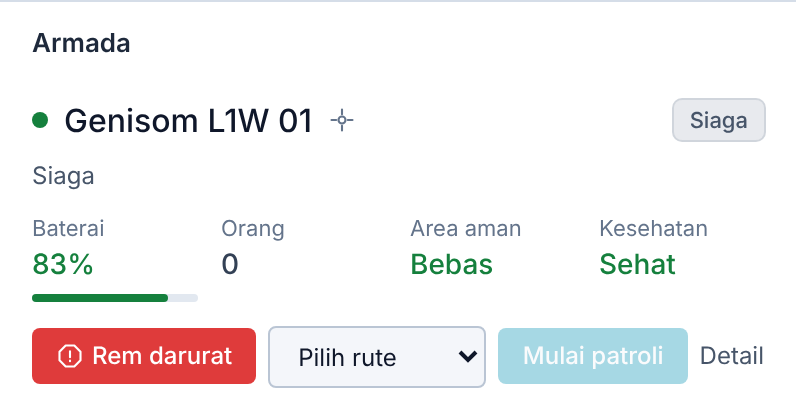
\includegraphics[width=\dimexpr\linewidth-1pt\relax]{img/robot-card-idle}}\\[3pt]
{\small\color{muted}Siaga: pilih rute lalu mulai}
\end{minipage}\hfill
\begin{minipage}[t]{0.48\linewidth}
\centering
\fcolorbox{line}{white}{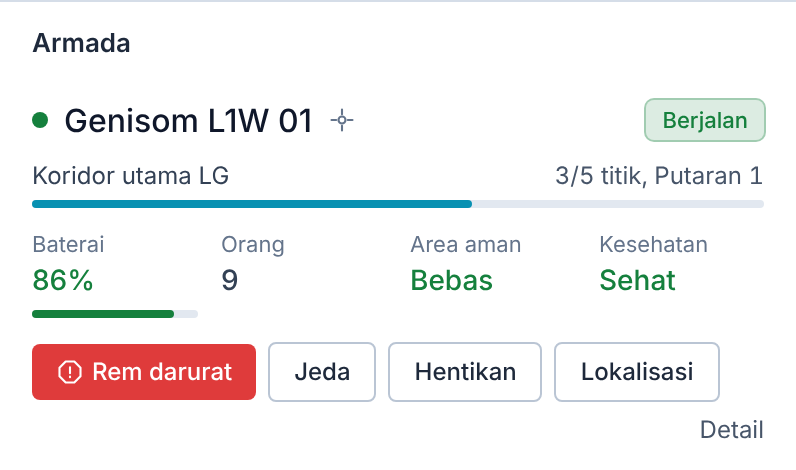
\includegraphics[width=\dimexpr\linewidth-1pt\relax]{img/robot-card-patrol}}\\[3pt]
{\small\color{muted}Sedang patroli}
\end{minipage}
\end{center}

\begin{tabularx}{\linewidth}{@{}B{3.4cm}Y@{}}
\toprule
Bagian & Arti \\
\midrule
Titik di depan nama & Hijau: robot tersambung ke NETRA. Abu-abu: tidak tersambung \\
Label kanan atas & Keadaan robot, misalnya \ui{Siaga}, \ui{Berjalan}, \ui{Inspeksi}, \ui{Dijeda}, \ui{Terhalang}, \ui{Rem darurat aktif} (tabel di bagian~\ref{sec:states}) \\
Rute dan kemajuan & Nama rute, titik stop yang sudah dilewati dan putaran ke berapa \\
Baterai & Kuning di bawah 25\,\%, merah di bawah 10\,\% \\
Orang & Jumlah orang yang terlihat kamera sekarang \\
Area aman & \ui{Bebas}, \ui{Melambat} (ada sesuatu di dekat robot), \ui{Berhenti} (terlalu dekat), \ui{Tanpa scan} (sensor tidak mengirim data, robot tidak boleh berjalan) \\
Kesehatan & \ui{Sehat}, atau jumlah masalah; arahkan mouse ke tulisan itu untuk detailnya \\
Tombol & \ui{Rem darurat}, \ui{Jeda}/\ui{Lanjutkan}, \ui{Hentikan}, \ui{Lokalisasi}; saat siaga \ui{Pilih rute} dan \ui{Mulai patroli}; \ui{Detail} membuka halaman robot \\
\bottomrule
\end{tabularx}

Klik nama robot untuk \ui{mengikuti} robot di peta: peta selalu berpusat pada robot itu. Tekan tanda
\ui{\texttimes} di label \ui{Mengikuti} untuk berhenti.

% ------------------------------------------------------------------------------------------ 6
\section{Menjalankan patroli}

\subsection{Memulai}
Pastikan langkah \hyperref[sec:prep]{persiapan} sudah dilakukan: robot online, berdiri, terlokalisasi,
handheld di AUTO dan rem darurat tidak aktif.

\begin{enumerate}
  \item Di \ui{Dasbor}, pada kartu robot, pilih rute di \ui{Pilih rute}.
  \item Tekan \ui{Mulai patroli}. Label berubah menjadi \ui{Berjalan} dan kemajuan rute mulai bergerak.
\end{enumerate}
Cara lain: menu \ui{Patroli} \ra{} panel \ui{Mulai patroli sekarang} (pilih robot dan rute, lalu
\ui{Mulai}); \ui{Jadwal} untuk patroli otomatis; atau dari handheld: \ui{Rute} \ra{} pilih rute
\ra{} \ui{Mulai}.

\subsection{Keadaan robot selama patroli}
\label{sec:states}
\begin{tabularx}{\linewidth}{@{}B{3.0cm}YY@{}}
\toprule
Label & Artinya & Yang dilakukan \\
\midrule
Berjalan & Menyusuri rute & Tidak perlu apa-apa \\
Menuju titik & Mendekati titik stop dengan pelan & -- \\
Inspeksi & Berhenti di titik stop, kamera dan AI memeriksa & -- \\
Selesai & Rute selesai & -- \\
Siaga & Tidak ada patroli & -- \\
Dijeda & Dihentikan sementara (\ui{Jeda}, atau rem darurat baru dilepas) & Tekan \ui{Lanjutkan} bila sudah aman \\
Terhalang & Ada orang atau barang di jalur, robot menunggu & Robot lanjut sendiri bila jalur bebas; minta orang memberi jalan atau singkirkan barang \\
Keluar rute & Robot terlalu jauh dari rute & \ui{Jeda}, bawa robot kembali ke rute dengan handheld (REMOTE), kembali ke AUTO, \ui{Lanjutkan} \\
Posisi hilang, Sensor macet & Robot tidak yakin posisinya, atau sensor berhenti mengirim data & \ui{Hentikan}, lokalisasi ulang lalu mulai lagi; bila terulang hubungi teknisi \\
Tanpa rute & Robot belum memuat rute & Mulai patroli dari NETRA \\
Rem darurat aktif & Rem darurat ditekan & Lihat bagian~\ref{sec:estop} \\
\bottomrule
\end{tabularx}

\subsection{Jeda, lanjutkan, hentikan}
\begin{itemize}
  \item \ui{Jeda}: robot berhenti di tempat dan mengingat posisinya di rute. \ui{Lanjutkan} meneruskan
        dari titik itu.
  \item \ui{Hentikan}: patroli berakhir (NETRA meminta konfirmasi). Riwayatnya tetap tersimpan.
  \item Patroli berakhir sendiri setelah semua putaran selesai. Pada rute berputar, robot juga
        mengakhiri putaran bila baterai lemah.
\end{itemize}

% ------------------------------------------------------------------------------------------ 7
\clearpage
\section{Peta operasi}
\shot{map}{Peta operasi dengan lapisan keramaian menyala}

\begin{itemize}
  \item \textbf{Lapisan} (kiri atas): \ui{Robot}, \ui{Rute}, \ui{Anomali} dan \ui{Keramaian (1 jam)}.
  \item \textbf{Tampilkan rute\ldots} (kanan atas): lihat rute mana pun di peta tanpa menjalankan
        patroli, misalnya untuk menjelaskan rute ke petugas baru.
  \item \textbf{Armada}, \textbf{Anomali} dan \textbf{Kejadian langsung} di kanan: keadaan robot,
        jumlah anomali yang perlu validasi, dan setiap kejadian begitu terjadi.
  \item Geser peta dengan menyeret, zoom dengan roda mouse atau dua jari, \ui{Pas} untuk melihat
        semuanya. Klik tanda anomali untuk membuka detailnya.
\end{itemize}

\begin{tips}[Peta grid]
Selama denah mall belum dipasang, peta berupa grid: satu kotak 1 meter, garis tebal tiap 5 meter.
Garis merah adalah sumbu x (arah depan robot saat peta pertama kali dibuat), garis hijau sumbu y, dan
titik 0,0 adalah tempat pemetaan dimulai. Setelah admin mengunggah dan mengkalibrasi denah di menu
\ui{Denah}, peta otomatis memakai denah mall.
\end{tips}

% ------------------------------------------------------------------------------------------ 8
\section{Rem darurat}
\label{sec:estop}

\subsection{Kapan ditekan}
\begin{itemize}
  \item Ada orang, terutama anak-anak, terlalu dekat dan robot tetap bergerak.
  \item Robot bergerak tidak wajar, menabrak, atau mendekati tangga, eskalator atau area terlarang.
  \item Ada keadaan darurat di area patroli (evakuasi, kebakaran, kerumunan besar).
\end{itemize}

\subsection{Saat rem darurat aktif}
\begin{center}
\begin{minipage}[t]{0.49\linewidth}
\centering
\fcolorbox{line}{white}{
\includegraphics[width=\dimexpr\linewidth-1pt\relax]{img/estop-attention}}\\[3pt]
{\small\color{muted}Muncul paling atas di \ui{Perlu perhatian}}
\end{minipage}\hfill
\begin{minipage}[t]{0.47\linewidth}
\centering
\fcolorbox{line}{white}{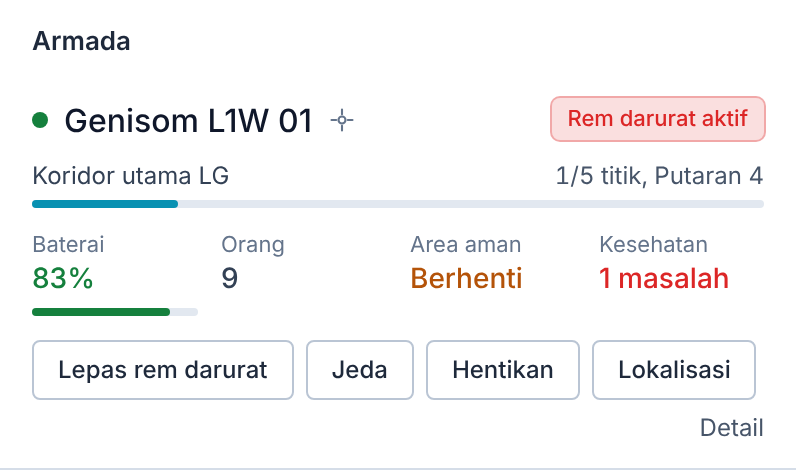
\includegraphics[width=\dimexpr\linewidth-1pt\relax]{img/robot-card-estop}}\\[3pt]
{\small\color{muted}Kartu robot: label merah, robot merah di peta}
\end{minipage}
\end{center}

\subsection{Melepas rem darurat}
\begin{enumerate}
  \item Pastikan penyebabnya sudah tertangani dan area di sekitar robot aman.
  \item NETRA: tekan \ui{Lepas rem darurat} lalu konfirmasi. Handheld: tahan tombol
        \ui{Tahan untuk lepas} selama satu detik.
  \item Robot sekarang \ui{Dijeda}. Tekan \ui{Lanjutkan} untuk meneruskan patroli, atau \ui{Hentikan}.
\end{enumerate}

\begin{penting}
Melepas rem darurat tidak langsung membuat robot berjalan. Patroli baru lanjut setelah seseorang
menekan \ui{Lanjutkan}, supaya tidak ada yang terkejut.
\end{penting}

% ------------------------------------------------------------------------------------------ 9
\clearpage
\section{Anomali dan validasi}

\subsection{Perjalanan sebuah anomali}
\begin{center}
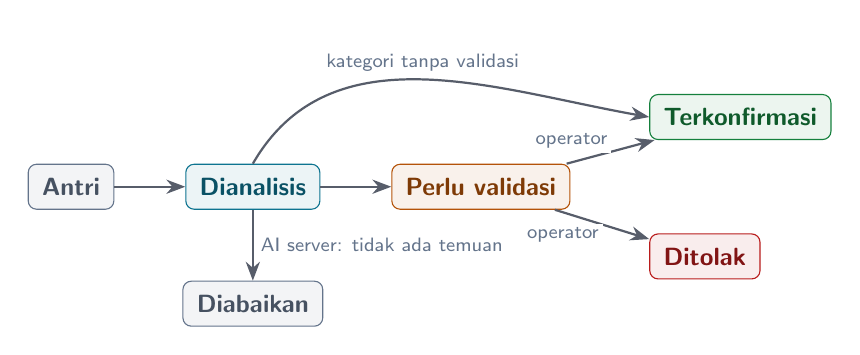
\begin{tikzpicture}[node distance=7mm and 9mm,every node/.style={align=center}]
  \node[state=muted] (q) {Antri};
  \node[state=netra,right=of q] (a) {Dianalisis};
  \node[state=warnc,right=of a] (n) {Perlu validasi};
  \node[state=okc,above right=3mm and 10mm of n] (c) {Terkonfirmasi};
  \node[state=dangerc,below right=3mm and 10mm of n] (r) {Ditolak};
  \node[state=muted,below=9mm of a] (d) {Diabaikan};
  \draw[arr] (q) -- (a);
  \draw[arr] (a) -- (n);
  \draw[arr] (n) -- node[lbl,above left=-1pt] {operator} (c);
  \draw[arr] (n) -- node[lbl,below left=-1pt] {operator} (r);
  \draw[arr] (a) -- node[lbl,right=1pt] {AI server: tidak ada temuan} (d);
  \draw[arr] (a.north) to[out=60,in=170] node[lbl,above=1pt] {kategori tanpa validasi} (c.west);
\end{tikzpicture}
\end{center}
\begin{itemize}
  \item \ui{Deteksi awal} adalah hasil AI di robot. \ui{Deteksi final} adalah hasil AI di server yang
        memeriksa ulang foto dengan lebih teliti (\ui{Dianalisis}).
  \item Kategori yang \emph{wajib validasi} menunggu operator (\ui{Perlu validasi}). Kategori tanpa
        validasi, misalnya sampah, langsung \ui{Terkonfirmasi} dan dikirim ke Telegram.
  \item Pengaturan per kategori (validasi, Telegram, grup tujuan, keyakinan minimum) ada di
        \ui{Pengaturan} \ra{} \ui{Aturan kategori anomali} (supervisor).
\end{itemize}

\subsection{Kategori}
\begin{tabularx}{\linewidth}{@{}B{3.0cm}YY@{}}
\toprule
Kategori & Contoh & Tindakan yang disarankan \\
\midrule
Sampah & Botol, gelas, kertas, plastik di lantai & Panggil cleaning service \\
Tumpahan & Minuman atau cairan di lantai & Pasang tanda lantai basah, panggil cleaning service \\
Lantai rusak & Keramik retak atau pecah, lubang & Beri tanda pengaman, lapor tim maintenance \\
\textcolor{dangerc}{Orang terjatuh} & Orang tergeletak di lantai & \textbf{Prioritas}: segera kirim petugas ke lokasi, ikuti prosedur P3K \\
Lainnya & Temuan lain & Lihat foto, tindak sesuai keadaan \\
\bottomrule
\end{tabularx}

\subsection{Memvalidasi}
\shot{anomaly-detail}{Detail anomali dengan formulir validasi}
\begin{enumerate}
  \item Buka \ui{Anomali} \ra{} tab \ui{Perlu validasi}, lalu klik kartunya. Bisa juga dari
        \ui{Perlu perhatian} di Dasbor.
  \item Perhatikan foto dan \ui{Hasil deteksi}: deteksi awal dan final, keterangan, posisi, patroli.
  \item Bila kategorinya salah, pilih yang benar di \ui{Kategori (ubah bila salah)}. Isi \ui{Catatan}
        bila perlu, misalnya ``sudah dibersihkan''.
  \item Tekan \ui{Konfirmasi} bila temuan benar, atau \ui{Tolak} bila salah (bayangan, pantulan,
        barang milik pengunjung yang diawasi).
\end{enumerate}
Setelah dikonfirmasi, NETRA mengirim foto ke grup Telegram kategori itu bila diatur; baris
\ui{Telegram} menunjukkan waktu kirimnya. Di Dasbor, anomali di \ui{Perlu perhatian} bisa langsung
dikonfirmasi atau ditolak tanpa membuka detail.

\subsection{Daftar anomali}
\shot{anomalies}{Daftar anomali: tab status, kategori, periode dan ekspor Excel}

% ------------------------------------------------------------------------------------------ 10
\clearpage
\section{Jadwal patroli}
\shot{schedules}{Daftar jadwal dan formulir jadwal baru}
\begin{enumerate}
  \item Buka \ui{Jadwal}. Isi panel \ui{Jadwal baru}: \ui{Nama} (misalnya Patroli pagi), robot dan rute.
  \item \ui{Ulangi}: \ui{Mingguan} lalu pilih hari, atau \ui{Sekali} lalu pilih tanggal.
  \item Isi \ui{Jam}. Jam mengikuti zona waktu pusat komando (WIB).
  \item Biarkan \ui{Aktif} menyala, lalu \ui{Simpan}.
\end{enumerate}
Ubah dengan \ui{Ubah}, matikan sementara dengan tombol geser, hapus dengan \ui{Hapus}. Kolom
\ui{Terakhir} menunjukkan kapan jadwal terakhir berjalan.

\begin{penting}
Pada jam jadwal, pusat komando dan robot harus menyala, robot berdiri dan terlokalisasi, handheld di
AUTO, dan rem darurat tidak aktif. Bila tidak, patroli tercatat \ui{Gagal} di menu Patroli.
\end{penting}

% ------------------------------------------------------------------------------------------ 11
\section{Rute}

\subsection{Basis data rute}
\shot{routes}{Rute terpilih ditampilkan di peta, titik stop bernomor}
Setiap rute yang direkam robot otomatis masuk ke menu \ui{Rute}. Klik rute untuk melihat jalurnya. Supervisor
dapat mengganti nama (\ui{Simpan nama}), menyembunyikan rute lama (\ui{Arsipkan}) dan mengunduh
file rute (\ui{Unduh CSV}).

\subsection{Merekam rute baru}
Dilakukan supervisor atau teknisi dengan handheld, sebaiknya saat mall sepi.

\begin{teknisi}
Robot harus dalam mode rekam: di robot isi \code{MODE=teach} pada \code{/etc/pashupati/pashupati.env},
lalu \code{sudo systemctl restart pashupati}. Setelah selesai merekam, kembalikan ke
\code{MODE=patrol} dan restart lagi.
\end{teknisi}

\begin{enumerate}
  \item Biarkan robot diam beberapa detik setelah menyala sampai siap.
  \item Di handheld pindah ke \ui{REMOTE}, lalu tekan \ui{Rekam}.
  \item Kemudikan robot pelan dan halus menyusuri jalur patroli.
  \item Di tempat robot harus berhenti dan memeriksa, berhentilah lalu tekan \ui{Titik}.
  \item Di depan setiap AprilTag, berhenti menghadap tag lalu tekan \ui{Tag}.
  \item Akhiri di dekat titik awal (untuk patroli berputar), lalu tekan \ui{Selesai}. Rute tersimpan
        dan muncul di NETRA \ra{} \ui{Rute}. Beri nama yang jelas, misalnya ``Koridor utama LG''.
\end{enumerate}

\begin{tips}[Rute yang baik]
Jaga jarak minimal 1 meter dari dinding dan etalase. Letakkan titik stop di tempat yang sering kotor:
food court, depan toilet, pintu masuk. Hindari rute yang melewati jalur paling padat pada jam sibuk.
\end{tips}

% ------------------------------------------------------------------------------------------ 12
\clearpage
\section{Riwayat patroli dan laporan}

\subsection{Patroli}
\shot{patrols}{Riwayat patroli dan panel mulai patroli}
Klik nomor patroli untuk membuka detailnya. Kolom \ui{PDF} mengunduh laporan patroli itu; \ui{Ekspor
Excel} mengunduh seluruh daftar.

\subsection{Detail patroli}
\shot{patrol-detail}{Ringkasan, peta rute dengan anomali, dan linimasa kejadian}
Di bagian atas: durasi, putaran, titik yang diinspeksi (dan yang dilewati), jumlah anomali dan puncak
keramaian. \ui{Linimasa} mencatat setiap kejadian: berangkat, tiba di titik, inspeksi selesai,
peringatan.

\subsection{Laporan}
\shot{reports}{Laporan untuk periode, robot dan bahasa pilihan}
Pilih \ui{Periode}, robot dan \ui{Bahasa laporan}, lalu unduh: \ui{Ringkasan operasi} (PDF atau
Excel), \ui{Daftar anomali} (Excel), \ui{Daftar patroli} (Excel). \ui{Laporan per patroli} lengkap
dengan foto ada di halaman Patroli.

% ------------------------------------------------------------------------------------------ 13
\clearpage
\section{Keramaian}
\shot{crowd}{Peta keramaian hari ini dan grafik per jam}
\begin{itemize}
  \item Warna kotak: biru dan hijau berarti sepi, kuning dan merah berarti ramai. Satu kotak 1 meter.
  \item \ui{Puncak} menampilkan jumlah tertinggi, \ui{Rata-rata} jumlah rata-rata. Pilih periode di
        kanan atas.
  \item Gunakan untuk mengatur jadwal patroli di luar jam ramai, atau menambah petugas di jam sibuk.
\end{itemize}

% ------------------------------------------------------------------------------------------ 14
\section{Halaman robot}
\begin{minipage}[t]{0.47\linewidth}
\vspace{0pt}\raggedright
Tekan \ui{Detail} di kartu robot. Di \ui{Kontrol langsung} (operator):
\begin{itemize}
  \item \ui{Inspeksi AI} nyala atau mati, \ui{Model} AI, dan \ui{Ritme}: \ui{Terus-menerus},
        \ui{Tiap n dtk}, atau \ui{Hanya titik stop}.
  \item \ui{Deteksi orang} nyala atau mati.
  \item \ui{Beban robot}: CPU, GPU, RAM dan suhu; merah bila 90\,\% atau lebih.
\end{itemize}
Perintah menunggu jawaban robot paling lama 10 detik; bila robot menolak, pesannya tampil merah.
Di bawahnya ada grafik beban, baterai dan orang, serta \ui{Putar ulang jalur} yang dilalui robot.
\end{minipage}\hfill
\begin{minipage}[t]{0.49\linewidth}
\vspace{0pt}\raggedright
\centering
\fcolorbox{line}{white}{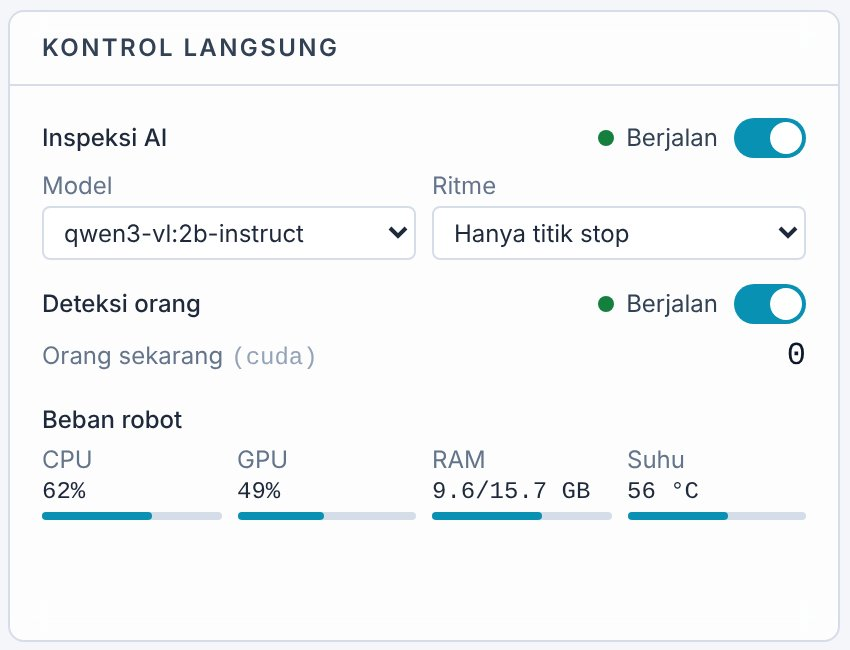
\includegraphics[width=\dimexpr\linewidth-1pt\relax]{img/robot-detail}}\\[3pt]
{\small\color{muted}Kontrol langsung}
\end{minipage}

% ------------------------------------------------------------------------------------------ 15
\section{Selesai bertugas}
\begin{enumerate}
  \item Pastikan tidak ada patroli berjalan (\ui{Hentikan} bila perlu) dan tidak ada anomali yang
        menunggu validasi.
  \item Bawa robot ke tempat parkir atau pengisian dengan handheld (REMOTE, pelan).
  \item Dudukkan robot: ikon \ui{Duduk} atau \key{L1}\,+\,\key{Y}.
  \item Matikan robot dan isi dayanya sesuai buku manual Genisom L1W.
  \item Isi daya handheld.
  \item Biarkan pusat komando menyala bila ada jadwal berikutnya. Di komputer bersama, keluar dari
        NETRA (ikon pintu di kiri bawah).
\end{enumerate}

% ------------------------------------------------------------------------------------------ 16
\clearpage
\section{Mengatasi masalah}
\begin{tabularx}{\linewidth}{@{}>{\raggedright\arraybackslash}p{4.2cm}>{\raggedright\arraybackslash}X>{\raggedright\arraybackslash}X@{}}
\toprule
\textbf{Masalah} & \textbf{Penyebab umum} & \textbf{Yang dilakukan} \\
\midrule
Robot tidak online (titik abu-abu) & Robot belum selesai menyala, beda Wi-Fi, atau pusat komando mati & Tunggu 3 menit; cek Wi-Fi; nyalakan ulang robot; hubungi teknisi \\
Patroli tidak mau mulai, atau \ui{Patroli gagal dimulai} & Belum lokalisasi, rem darurat aktif, handheld di REMOTE, robot jauh dari rute & Lokalisasi, lepas rem darurat, pindah ke AUTO, dekatkan robot ke rute \\
\ui{Terhalang} lama & Orang atau barang tetap di jalur & Minta orang memberi jalan, singkirkan barang \\
\ui{Keluar rute} & Robot terdorong atau terlalu jauh dari rute & Jeda, kembalikan ke rute dengan handheld, AUTO, Lanjutkan \\
\ui{Posisi hilang}, \ui{Sensor macet}, \ui{Pemindaian keselamatan macet} & Sensor atau perhitungan posisi bermasalah & Hentikan, lokalisasi ulang; bila terulang nyalakan ulang robot dan hubungi teknisi \\
\ui{Baterai lemah} & Baterai di bawah 25\,\% & Akhiri patroli, kembalikan robot, isi daya \\
\ui{Koneksi terputus saat patroli} & Robot keluar dari jangkauan Wi-Fi & Cari robot di rute; dekatkan ke access point; hubungi teknisi bila sering \\
Anomali lama di \ui{Dianalisis} & AI server sibuk atau sedang memuat model & Tunggu; bila lebih dari 10 menit hubungi teknisi \\
Handheld: \ui{token ditolak} & Token di aplikasi dan di robot berbeda & Hubungi teknisi \\
Handheld: \ui{robot tidak menjawab} & Handheld di Wi-Fi lain, atau robot mati & Cek Wi-Fi handheld, nyalakan robot \\
Handheld tersambung tapi robot tidak berjalan & Mode AUTO, atau rem darurat aktif & Pindah ke REMOTE, lepas rem darurat \\
NETRA \ui{Terputus} (titik merah di atas) & Koneksi komputer ke NETRA putus & Cek jaringan, muat ulang halaman \\
Telegram tidak masuk & Telegram belum diatur, atau kategori tidak dikirim & Hubungi admin \\
\ui{Jam robot selisih \ldots} & Jam robot belum sinkron & NETRA sudah mengoreksi waktu; beri tahu teknisi \\
Lupa kata sandi & -- & Minta admin mereset di \ui{Pengguna} \\
\bottomrule
\end{tabularx}

% ------------------------------------------------------------------------------------------ appendix
\clearpage
\appendix
\renewcommand{\thesection}{\Alph{section}}
\section{Tombol handheld}
\begin{tabularx}{\linewidth}{@{}B{4.6cm}YY@{}}
\toprule
Fungsi & Gamepad & Layar sentuh \\
\midrule
Maju, mundur, geser & Stik kiri & -- \\
Belok & Stik kanan & -- \\
\textcolor{dangerc}{STOP (rem darurat)} & \key{B}, di semua halaman & Tombol merah \\
Lepas rem darurat & -- & Tahan \ui{Tahan untuk lepas} 1 detik \\
AUTO / REMOTE & \key{Start} & Saklar di atas \\
Tukar kamera dan peta & \key{Select} & Ketuk tampilan kecil \\
Gigi kecepatan (30, 60, 100\,\%) & D-pad atas / bawah & \ui{Pengaturan}, Kecepatan \\
Berdiri / Duduk & \key{L1}\,+\,\key{A} / \key{L1}\,+\,\key{Y} & Ikon di bawah STOP \\
Peta & -- & Cubit untuk zoom, seret, putar; ketuk dua kali untuk mengikuti robot \\
\bottomrule
\end{tabularx}

Ikon patroli di layar utama: \ui{Rekam}, \ui{Titik}, \ui{Tag}, \ui{Selesai} (merekam rute),
\ui{Lokasi} (lokalisasi), \ui{Rute} (pilih rute), \ui{Mulai}, \ui{Jeda}, \ui{Lanjut}, \ui{Akhiri}.
Robot hanya mengikuti stik di mode REMOTE; di mode AUTO, navigasi yang mengemudikan.

\section{Istilah}
\begin{tabularx}{\linewidth}{@{}B{3.6cm}Y@{}}
\toprule
Istilah & Arti \\
\midrule
Rute & Jalur patroli yang direkam sekali lalu diulang robot \\
Titik stop & Tempat di rute untuk berhenti dan memeriksa lantai \\
Putaran & Satu kali menyelesaikan rute; rute berputar bisa diulang beberapa putaran \\
AprilTag & Kertas bermotif kotak hitam-putih di dinding; dari tag ini robot tahu posisinya \\
Lokalisasi & Robot menentukan posisinya di peta dengan melihat AprilTag \\
AUTO / REMOTE & AUTO: robot berpatroli sendiri. REMOTE: robot mengikuti stik handheld \\
Rem darurat (e-stop) & Menahan robot diam sampai dilepas dengan sengaja \\
Area aman & Daerah di sekeliling robot; robot melambat atau berhenti bila ada yang terlalu dekat \\
Anomali & Temuan robot: sampah, tumpahan, lantai rusak, orang terjatuh, lainnya \\
Deteksi awal / final & Hasil AI di robot / hasil AI di server yang memeriksa ulang \\
Validasi & Petugas memastikan anomali benar (Konfirmasi) atau salah (Tolak) \\
Grid & Peta kotak-kotak 1 meter yang dipakai selama denah mall belum dipasang \\
\bottomrule
\end{tabularx}

\clearpage
\section{Untuk admin dan teknisi}
\subsection*{Pengguna}
\ui{Pengguna} \ra{} \ui{Tambah pengguna}: nama pengguna, nama tampilan, peran, kata sandi minimal
8 karakter. Di daftar: ganti peran, \ui{Reset kata sandi}, \ui{Nonaktifkan} atau \ui{Hapus}.

\subsection*{Menambah robot}
\begin{enumerate}
  \item \ui{Pengaturan} \ra{} \ui{Robot}: isi \ui{ID robot} (misalnya \code{l1w-01}) dan nama, lalu
        \ui{Tambah}.
  \item Salin \code{CC\_URL} dan \code{CC\_TOKEN} yang tampil (token hanya ditampilkan sekali).
  \item Di robot, isi keduanya beserta \code{ROBOT\_ID} di \code{/etc/pashupati/pashupati.env}, lalu
        \code{sudo systemctl restart pashupati}. Robot muncul online dalam satu menit.
\end{enumerate}

\subsection*{Aturan anomali dan klien API}
\ui{Pengaturan} \ra{} \ui{Aturan kategori anomali}: per kategori atur \ui{Validasi}, \ui{Telegram},
\ui{Chat ID} grup tujuan dan \ui{Min. yakin}. \ui{Klien API} (admin) memberi aplikasi pihak ketiga
akses baca ke anomali beserta fotonya; dokumentasinya di \code{/api/ext/docs}.

\subsection*{Pusat komando di laptop}
\begin{teknisi}[Perintah di folder Netra (Mac)]
\begin{tabular}{@{}ll@{}}
\code{scripts/local.sh start} & menyalakan tanpa internet (hari demo) \\
\code{scripts/local.sh up} & menyalakan atau memperbarui \\
\code{scripts/local.sh status} & keadaan layanan \\
\code{scripts/local.sh lan} & alamat laptop untuk \code{CC\_URL} robot dan HP \\
\code{scripts/local.sh down} & mematikan (data tetap tersimpan) \\
\end{tabular}

Selengkapnya: \code{LOCAL.md} dan \code{README.md} di repositori Netra.
\end{teknisi}

% ------------------------------------------------------------------------------------------ card
\clearpage
\section{Kartu ringkas}
\label{sec:kartu}
\begin{multicols}{2}
\subsection*{Mulai shift}
\begin{enumerate}
  \item Buka NETRA, login, pilih \ui{ID}.
  \item Cek area patroli aman dan kering.
  \item Nyalakan robot, tunggu titik hijau di NETRA.
  \item Handheld: pilih robot, \ui{Berdiri}.
  \item REMOTE: bawa robot ke titik awal, hadap AprilTag.
  \item \ui{Lokalisasi} (NETRA) atau \ui{Lokasi} (handheld).
  \item Handheld kembali ke \ui{AUTO}.
  \item Dasbor: \ui{Pilih rute} \ra{} \ui{Mulai patroli}.
\end{enumerate}

\subsection*{Selama patroli}
\begin{itemize}
  \item Pantau \ui{Perlu perhatian} di Dasbor.
  \item Validasi anomali: \ui{Konfirmasi} atau \ui{Tolak}.
  \item \textcolor{dangerc}{\textbf{Orang terjatuh}}: kirim petugas sekarang.
  \item \ui{Terhalang}: bantu buka jalur.
\end{itemize}

\columnbreak
\subsection*{Darurat}
\begin{penting}[Rem darurat]
NETRA: \ui{Rem darurat}. Handheld: \ui{STOP} atau \key{B}.\\[3pt]
Lepas hanya bila aman: \ui{Lepas rem darurat}, lalu \ui{Lanjutkan}.
\end{penting}

\subsection*{Akhir shift}
\begin{enumerate}
  \item Tidak ada patroli berjalan dan anomali tertunda.
  \item Bawa robot ke tempat parkir, \ui{Duduk}.
  \item Matikan dan isi daya robot dan handheld.
  \item Keluar dari NETRA.
\end{enumerate}

\subsection*{Kontak}
\renewcommand{\arraystretch}{1.9}
\begin{tabular}{@{}l p{4.2cm}@{}}
Teknisi & \hrulefill \\
Supervisor & \hrulefill \\
Cleaning service & \hrulefill \\
Alamat NETRA & \hrulefill \\
\end{tabular}
\end{multicols}

\end{document}
